\section{Introducci�n}


\subsection{Radio definida por software (SDR)}

El concepto de Radio Definida por Software se le atribuye a Joseph Mitola, 1990. Se refiere a un dispositivo que permite reducir al m�nimo el hardware necesario para la recepci�n de se�ales de radio. Dicho equipo captura la se�al anal�gica (ya sea mediante un cable o una antena), la digitaliza (mediante un conversor A/D) para luego realizar por software toda la etapa de procesamiento de se�al requerido en la decodificaci�n. Esto ha logrado que la recepci�n de cierto rango de telecomunicaciones sea mucho m�s accesible en t�rminos econ�micos y pr�cticos (ya que el mismo dispositivo f�sico se puede utilizar para distintos fines con solo re-programar el software). Un ejemplo de este dispositivo se puede ver a continuaci�n:

\begin{figure}[H]
\begin{centering}
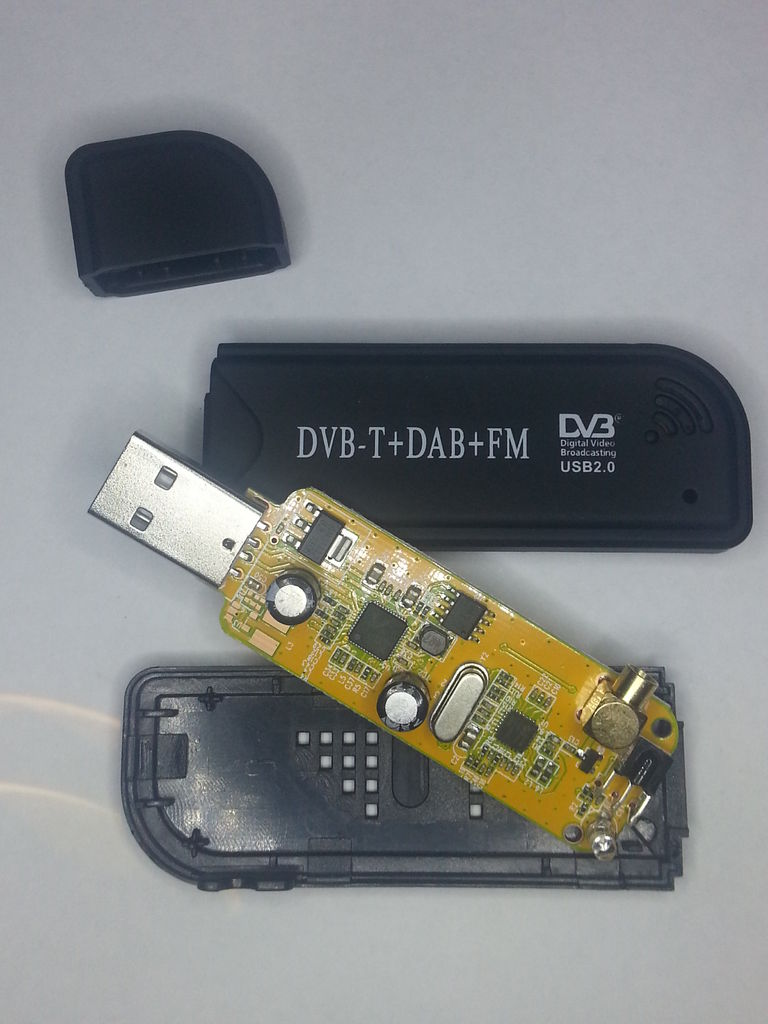
\includegraphics[width=0.75\textwidth]{SDR.jpg}
\par\end{centering}

\caption{Sintonizador de radio digital.}


\end{figure}



\subsection{Transmisi�n de TV por cable}

En telecomunicaciones, la televisi�n anal�gica se transmite mediante
el m�todo de la Multiplexi�n por Divisi�n en Frecuencia (FDM). Esta
t�cnica consiste en transmitir varias se�ales simult�neamente modulando
cada una con una portadora diferente, en el rango de VHF/UHF, de forma
tal que los anchos de banda de cada se�al no se superpongan significativamente.
El canal destinado para la transmisi�n de una emisora tiene un ancho
de banda de aproximadamente 6 Mhz, donde los 5.45 Mhz m�s bajos corresponden
al espectro de la se�al de video y los �ltimos 0.55Mhz (aproximadamente)
se reservan para el espectro de la se�al de audio. Este modelo de
comunicaci�n se puede ver representado en el siguiente gr�fico:

\begin{figure}[H]
\begin{centering}
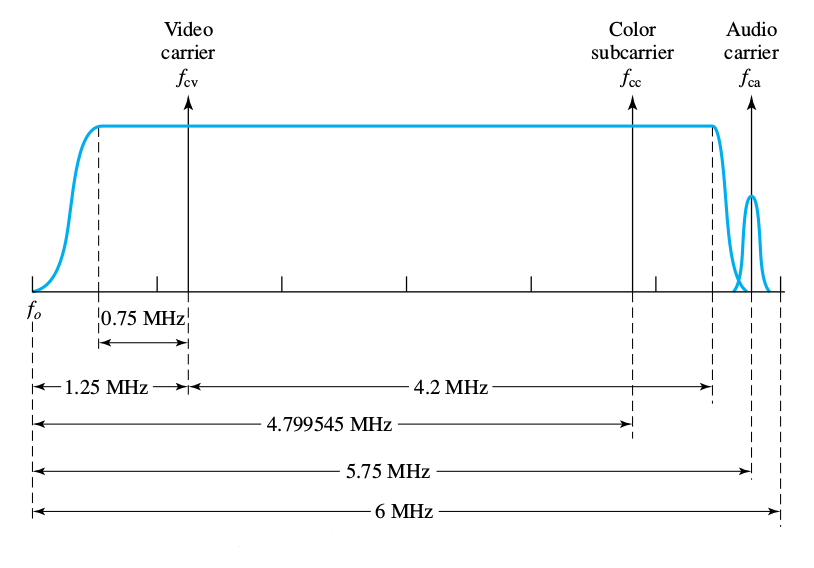
\includegraphics[width=0.75\textwidth]{TV_Spectrum.png}
\par\end{centering}

\caption{Se�al de TV transmitida.}
\end{figure}



\subsection{Aplicaci�n del Trabajo Pr�ctico}

Sabiendo que el audio de la televisi�n est� modulado en frecuencia
(FM), si se toma la porci�n del canal adecuada es posible demodular
dicha se�al y escuchar alg�n canal de televisi�n.

En este caso particular, el SDR se utiliz� para capturar un ancho
de banda de 2.4Mhz y centrado en 181.238 Mhz. A trav�s del aplicativo
desarrollado se pudo escuchar efectivamente el programa emitido.

